\chapter{Documentos HTML e CSS}

Este capítulo aborda a estrutura básica dos de documentos HTML e CSS. Veremos como é a hierarquia de elementos de um documento HTML, como se cria um novo elemento, o que são \textit{tags}, atributos e valores de atributos. Veremos também como é o código de um documento CSS básico, com seletores e propriedades para formatação visual de elementos específicos.

\section{Estrutura de Uma Página HTML}

Uma página HTML também pode ser chamada de documento HTML. O exemplo \ref{code_html} mostra o código de um documento HTML de uma página bem simples. Vale ressaltar que os números das linhas foram colocados só para facilitar a explicação. Eles não fazem parte do código do documento HTML.

\begin{htmlcode}{O código de uma página HTML simples}{code_html}
<!DOCTYPE html>
<html lang="pt-br">
   <head>
      <meta charset="UTF-8">
      <meta name="viewport" content="width=device-width, initial-scale=1.0">
      <title>Título do Site</title>
   </head>
   <body>
      <h1>Título da Página</h1>
      <p>Id culpa velit deserunt ullamco veniam. Occaecat aute voluptate    
       sint ut magna. Veniam consequat pariatur dolore eu sit ea.</p>
   </body>
</html>
\end{htmlcode}

Agora nós vamos analisar detalhadamente os elementos que fazem parte desse documento HTML. Você vai precisar desse conhecimento para todo o restante de sua jornada como desenvolvedor web, portanto, preste bastante atenção. 

Os documentos HTML possuem uma estrutura básica que está presente em todos eles. Um documento HTML é composto por elementos. Alguns tipos de elementos podem conter outros elementos. Quando possuem essa capacidade, esses elementos podem ser chamados de elementos contêiner.

Um elemento contêiner é delimitado por uma tag de abertura e uma tag de fechamento. Temos alguns elementos contêineres aqui no exemplo \ref{code_html}. Vamos ver quais são. Temos o elemento \var{html}, que inicia na linha 2 e termina na linha 13; o elemento \var{head}, que inicia na linha 3 e termina na linha 7; o elemento \var{body}, que começa na linha 8 e termina na linha 12; o elemento \var{title}, que começa e termina na linha 6; o elemento \var{h1}, com início e fim na linha 9; e o elemento \var{p}, que inicia na linha 10 e termina na linha 11. 

Quando um elemento não pode conter outros elementos, ele é chamado de elemento simples e possui apenas a \textit{tag} de abertura. Isso acontece com o elemento \var{DOCTYPE}, na linha 1, e com os elementos \var{meta}, nas linhas 4 e 5. Veja que são dois elementos distintos.

Uma \textit{tag}, por sua vez, corresponde a uma ou mais palavras envolvidas pelos símbolos de menor e maior (\var{<tag>}). A \textit{tag} de abertura pode conter mais de uma palavra, sendo que a primeira palavra corresponde ao tipo de elemento \var{html} dessa \textit{tag} e as demais palavras nós veremos daqui a pouco. 

Na \textit{tag} de abertura da linha 4, por exemplo, a primeira palavra é \var{meta}, ou seja, esse é um elemento \var{html} do tipo \var{meta}. A \textit{tag} de fechamento sempre terá somente o nome do tipo de elemento \var{html} precedido por uma barra (\var{</tag>}). Vamos identificar as \textit{tags} de fechamento desse documento HTML. 

No final da linha 6 temos o fechamento de um elemento do tipo \var{title}. No final da linha 7 temos o fechamento do elemento \var{head}. No final da linha 9 temos o fechamento do elemento do tipo \var{h1}. No final da linha 11 temos o fechamento de um elemento do tipo \var{p}. Na linha 12 temos o fechamento do elemento \var{body}, e na linha 13 temos o fechamento do elemento \var{html}.

Agora que já sabemos identificar as tags de abertura e de fechamento dos elementos, vamos analisar um pouco melhor os tipos de elemento presentes nessa página e suas tags de abertura. Na linha 1, temos o elemento \var{DOCTYPE}, que é um elemento simples, ou seja, ele tem somente a \textit{tag} de abertura. O elemento \var{DOCTYPE} existe apenas para indicar ao navegador que esse é um documento HTML. 

O elemento \var{DOCTYPE} sempre aparece no início do documento e seu uso é recomendado, apesar de sua ausência não causar nenhum erro de renderização de página nos navegadores atuais. Veja que dentro da \textit{tag} \var{DOCTYPE} temos mais uma palavra, que é \var{html}. Essa palavra é um atributo. Portanto, elementos podem conter atributos em suas \textit{tags} de abertura. Nunca teremos atributos dentro de uma \textit{tag} de fechamento.

Esse ponto de exclamação que vem antes do nome do elemento \var{DOCTYPE} é um resquício histórico usado em versões antigas. Somente esse elemento inicia com esse ponto de exclamação. O elemento \var{DOCTYPE} vai aparecer desse jeito em qualquer documento HTML atual, porque esse é o padrão para indicar que se trata de um documento HTML 5.

Na linha 2, temos a tag de abertura de um elemento do tipo \var{html}. Observe que esse elemento é fechado na linha 13. Portanto, todos os elementos que estão entre as linhas 2 e 13 são filhos, netos, bisnetos ou algum outro descendente do elemento \var{html}. 

Veja também que o elemento \var{html} possui o atributo \var{lang} em sua \textit{tag} de abertura, mas esse atributo tem uma forma diferente do atributo \var{html} presente na \textit{tag} da linha 1. Acontece que o atributo da linha 2 possui um valor, enquanto o atributo da linha 1 apenas existe.

Em algumas poucas situações, a simples existência de um atributo em uma \textit{tag} é suficiente para se definir alguma configuração. Na maioria das situações, os atributos são acompanhados de um valor, como é o caso do atributo da linha 2. Nesse caso, o atributo \var{lang} tem o valor \var{pt-br}. O valor do atributo \var{lang} da \textit{tag} \var{html} define o idioma predominante do conteúdo do documento HTML em questão. 

Isso é importante para que o navegador exiba caracteres internacionais corretamente e também para que ferramentas de busca, como o Google, identifiquem mais facilmente que esse site tem mais relevância para pessoas que falam o idioma Português do Brasil, nesse caso.

Um documento HTML só pode ter 1 único elemento do tipo \var{html}. Ele é o elemento ancestral de todos os demais elementos da página, exceto do elemento \var{DOCTYPE}. Todos os elementos que estiverem entre as \textit{tags} de abertura e de fechamento de um elemento contêiner, são considerados elementos filhos desse elemento contêiner. Elementos que são filhos de filhos são considerados elementos netos, e assim por diante.

Veja que a linha 3 tem um elemento contêiner do tipo \var{head}, que é fechado na linha 7. Assim como acontece com o elemento \var{html}, um documento HTML também só pode ter 1 elemento do tipo \textit{head}. O elemento \var{head} contém metainformações relacionadas ao documento em questão, ou seja, os elementos dentro de \var{head} não correspondem a conteúdo, mas sim a informações sobre o próprio documento HTML, portanto, não são renderizados pelo navegador.

Alguns elementos de metainformações até podem ter influência no visual de elementos de conteúdo que são renderizados pelo navegador, mas eles próprios jamais serão renderizados pelo navegador. Dentro do elemento \var{head}, na linha 4, temos um elemento de metainformação que indica qual é o conjunto de caracteres que deve ser utilizado para mostrar textos nessa página. Nesse caso, está sendo usado o \var{utf-8}, que é o padrão para idiomas ocidentais.

O elemento de metainformação da linha 5, que também está dentro de \var{head}, parece meio assustador, mas não precisa se preocupar em entendê-lo plenamente nesse momento. A princípio, basta saber que ele define uma configuração para a exibição correta da página em dispositivos com diferentes tamanhos de tela.

Na linha 6 temos o elemento \var{title}. Esse elemento define o título da página mostrado na aba do navegador. É por isso que esse elemento fica dentro de \var{head}, porque ele não é considerado conteúdo. Vale observar que não faz sentido colocar dois ou mais elementos \var{title} em um documento HTML. Portanto, só temos 1 elemento \var{title} por documento.

Agora vamos ao elemento da linha 8. É dentro dele que tudo acontece. O elemento \var{body}, que é fechado na linha 12 nesse caso, envolve todos os elementos de conteúdo de um documento HTML. Assim como os elementos \var{html}, \var{head} e \var{title}, um documento HTML só tem um elemento \var{body}. Nesse caso nós temos simplesmente um elemento do tipo \var{h1}, que representa um título, e um elemento do tipo \var{p}, que representa um parágrafo.

Ao longo do curso, veremos todos os tipos de elementos HTML que podem ser colocados dentro do elemento \var{body}, incluindo vários níveis de título, parágrafos, tabelas, links, imagens, formulários, entre outros. Vamos relembrar alguns pontos importantes que aprendemos com esse documento HTML. Com exceção dos elementos entre as linhas 9 e 11, todos os demais elementos desse exemplo estão presentes em todas as páginas web.

Em síntese, um documento HTML é composto por um único elemento \var{html}, que por sua vez que contém um elemento \var{head} e um elemento \var{body}. O elemento \var{head}, por sua vez, contém alguns elementos de metainformações e um elemento do tipo \var{title}. Ao longo do curso, veremos outros elementos que podem aparecer dentro do elemento \var{head}. Já o elemento \var{body} é o que contém todos os elementos correspondentes ao conteúdo da página, os quais também veremos em capítulos posteriores.

O exemplo \ref{code_html_simples} mostra o código de uma página HTML realmente simples, enquanto a figura \ref{fig:rend_html_simples} mostra como esse código é renderizado no navegador. O importante aqui é que você perceba que um documento HTML escrito puramente com código HTML, geralmente tem essa aparência sem graça. Se quisermos melhorar a aparência desse documento, temos que fazer uso de CSS. Apesar de ainda estarmos na parte de HTML, a próxima seção apresenta como é a estrutura básica de um documento CSS e como ele se relaciona com um documento HTML.

\begin{htmlcode}{Documento HTML simples}{code_html_simples}
<!DOCTYPE html>
<html lang="pt-br">
<head>
    <meta charset="UTF-8">
    <meta name="viewport" content="width=device-width, initial-scale=1.0">
    <title>Título do Site</title>
</head>
<body>
    <header>
        <h1>Título da Página</h1>
        <hr>
    </header>
    <main>
        <h2>Subtítulo 1</h2>
        <p>Cupidatat esse ipsum ad occaecat. Incididunt fugiat culpa ame 
            illum veniam reprehenderit reprehenderit in ad.</p>
        <h2>Subtítulo 2</h2>
        <p>Deserunt proident amet Lorem tempor fugiat ad elit laborum sit 
            officia consectetur.</p>    
    </main>
    <footer>
        <hr>
        <p>
            Copyright &copy; 2021 :: Todos os direitos reservados
        </p>
    </footer>    
</body>
</html>
\end{htmlcode}

\begin{figure}[ht!]
    \centering
    \frame{
    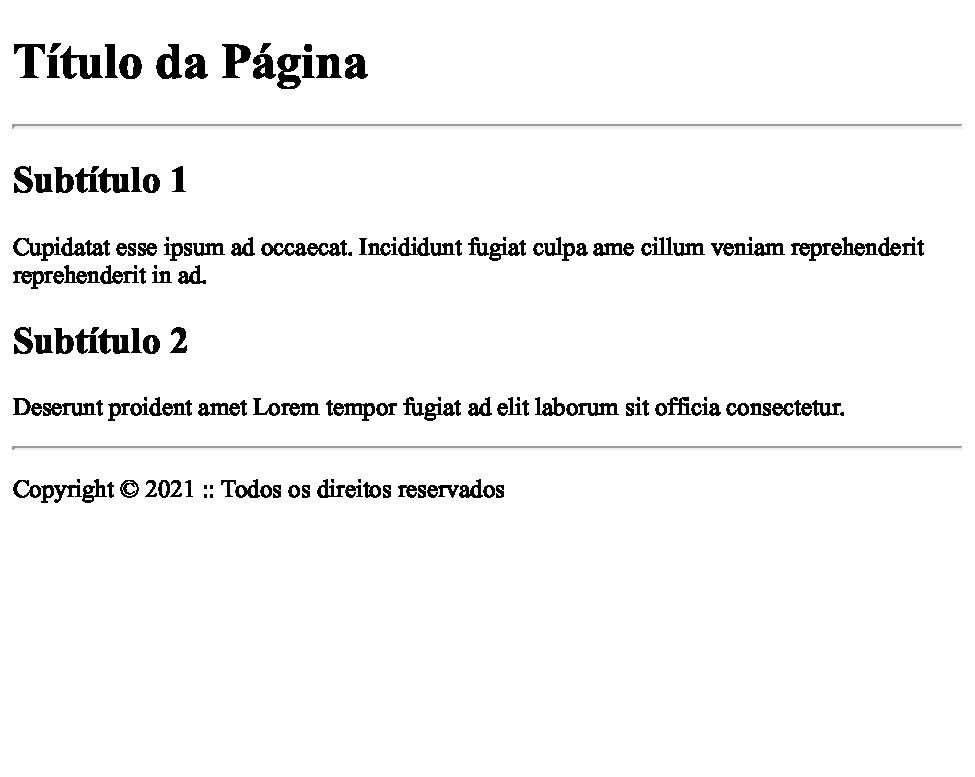
\includegraphics[width=1\textwidth, trim={0 4cm 0 0}]{Images/chapter02/html_simples.pdf}}
    \caption{Renderização do código HTML do exemplo \ref{code_html_simples}.}
    \label{fig:rend_html_simples}
\end{figure}

\section{Estrutura de Um Documento CSS}

O exemplo \ref{code_css_simples} apresenta um código CSS bem simples. Nós não nos aprofundaremos no estudo de CSS agora, porque o foco da parte I deste material é HTML. Entretanto, é importante você já saber como um documento CSS se relaciona com um documento HTML.

\begin{csscode}{Documento CSS simples}{code_css_simples}
body {
    font-family: 'Segoe UI', Tahoma, Geneva, Verdana, sans-serif;
    padding: 50px;
    background-color: lightgray;
}
h1 {
    color: darkgray;
    text-align: center;
    border: solid 1px black;
}
p {
    text-align: justify;
    font-size: 16px;
}
\end{csscode}

Um documento CSS contém uma série de seletores. Um \textbf{seletor} é composto por um \textbf{identificador} e por um bloco de \textbf{propriedades}, sendo que esse bloco é delimitado por abertura e fechamento de chaves. Esse documento CSS tem 3 seletores: o seletor \var{body}, que vai da linha 1 à linha 5; o seletor \var{h1}, da linha 6 a 10; e o seletor \var{p}, da linha 11 a 14.

O identificador de um seletor deve ser único no documento. Esse identificador pode ser criado de diferentes formas, sendo que cada forma atinge um ou vários elementos HTML. Nesse caso, estamos usando seletores por tipo, ou seja, os nomes dos seletores usados nesse exemplo coincidem com alguns tipos de elementos HTML que vimos na seção anterior.

Um seletor cujo identificador coincide com o nome de um tipo de elemento define o estilo do tipo de elemento HTML em questão. Existem outras formas de seletores, como o seletor por ID e o seletor por classes. Também existem seletores que são combinações desses 3 tipos. Mais adiante, teremos um tópico só para tratar de seletores, portanto, não se preocupe em tentar entender completamente o funcionamento dos seletores agora.

Nesse código CSS do exemplo \ref{code_css_simples}, de acordo com as propriedades definidas pelo seletor \var{h1} que inicia na linha 6, o elemento do tipo \var{h1} terá cor de fonte cinza escura, alinhamento de texto centralizado e uma borda sólida de 1 pixel na cor preta. 

Os outros seletores definem outras propriedades visuais para os elementos \var{body} e \var{p}. Algumas propriedades definidas para elementos do tipo contêiner podem afetar os elementos filhos, como é o caso da propriedade font-family do seletor \var{body}, na linha 2. Esse seletor define uma lista de fontes de letra para que o documento use a primeira que estiver disponível dessa lista. Como mencionei, existem várias formas de se construir seletores e várias propriedades que podem ser configuradas. Estudaremos mais sobre isso ao longo deste material.

\subsection{Associando um Documento CSS a um Documento HTML}

Esta seção mostra como associar o código CSS do exemplo \ref{code_css_simples} ao código HTML do exemplo \ref{code_html_simples}. Vale ressaltar que esta não é a única forma de se aplicar definições CSS a um documento HTML, porém, é a forma mais usual. Outras formas de associação são mostradas na parte II deste material. A associação de um documento CSS a um documento HTML é algo relativamente simples de se fazer. O exemplo \ref{code_ref_css} mostra um trecho de código que contém a associação de um documento CSS chamado ``estilos.css'' a um documento HTML qualquer. 

\begin{csscode}{Associação de documento CSS a um documento HTML}{code_ref_css}
<head>
    ...
    <title>Título do Site</title>
    <link rel="stylesheet" href="estilos.css">
</head>
\end{csscode}

Como pode ser visto na linha 4, basta usar um elemento do tipo \var{link} dentro do elemento \var{head} da página, e definir o valor do atributo \var{rel} como \var{stylesheet} e o valor do atributo \var{href} com o nome do arquivo CSS que deseja vincular a esse documento HTML. Nesse caso, o nome arquivo é ``estilos.css''. Vale ressaltar é possível ter vários documentos CSS associados a um único documento HTML, bem como um mesmo documento CSS associado a vários documentos HTML, e isso é bem comum.

Usar um único arquivo CSS (ou um conjunto de arquivos CSS) para todas as páginas de um site pode facilitar bastante a alteração do visual inteiro do site sem muito esforço, como veremos mais adiante na segunda parte deste material. Agora vamos ver na figura \ref{fig:rend_html_com_css} o resultado da associação desse documento CSS ao documento HTML simples cujo código corresponde ao do exemplo \ref{code_html_simples}.

\begin{figure}[htbp!]
    \centering
    \frame{
    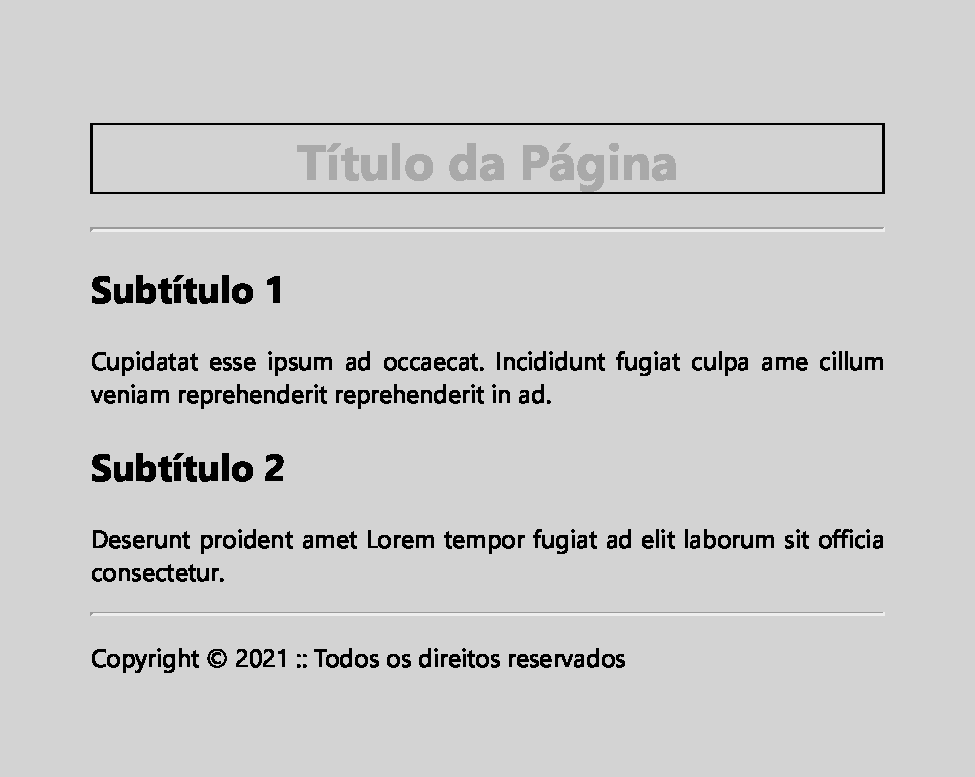
\includegraphics[width=1\textwidth]{Images/chapter02/html_com_css.pdf}}
    \caption{Renderização do código HTML do exemplo \ref{code_html_simples} com o CSS do exemplo \ref{code_css_simples} associado.}
    \label{fig:rend_html_com_css}
\end{figure}

Certamente a renderização com a aplicação do CSS neste caso não melhorou muito, mas o objetivo aqui é só de mostrar que o CSS afetou o visual da página. Com certeza muita coisa poderia ser configurada via CSS neste documento HTML para deixá-lo com o visual bastante profissional. Veremos os recursos necessários para isso ao longo deste material.

\section{Exercícios Propostos}

Essa série de exercícios envolve os conceitos abordados neste capítulo e também \textbf{pode demandar alguma pesquisa}. Reserve um tempo e um local adequados para fazer os exercícios sem distrações. Assim você absorverá muito mais o conteúdo estudado.

\begin{exercise}
Qual é o elemento HTML que contém todos os demais elementos de uma página?
\end{exercise}

\begin{exercise}
Qual é o elemento HTML que contém elementos com metainformações sobre uma página web?
\end{exercise}

\begin{exercise}
Qual é o elemento HTML que contém todos os elementos de conteúdo de uma página web?
\end{exercise}

\begin{exercise}
Qual é o elemento HTML que permite associar um documento CSS a uma página web na seção de metainformações?
\end{exercise}

\section{Considerações Sobre o Capítulo}

Este capítulo apresentou a estrutura básica dos documentos HTML e dos documentos CSS. Vimos quais são os principais elementos comumente presentes na hierarquia de elementos da maioria dos documentos HTML. Vimos também como criar e um documento CSS com propriedades que configuram elementos de acordo com seu tipo e como associar tal documento a um documento HTML qualquer. No capítulo seguinte, iniciaremos o estudo da linguagem HTML em si e seus elementos textuais básicos.